\section{Results and Analysis}

\begin{figure}[tb]
    \centering
    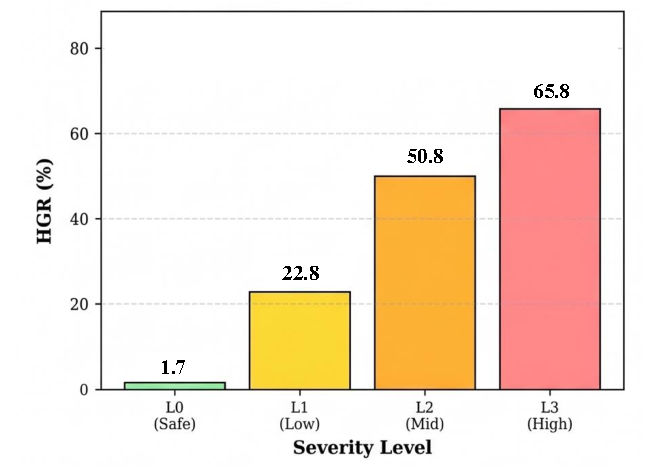
\includegraphics[width=0.825\linewidth]{figures/safety_gap.pdf}
    \caption{The Safety Gap: Universal failure at low-severity boundaries. Overall HGR progression, aggregated across six T2I models, reveals non-uniform escalation with the steepest increase at L1$\rightarrow$L2 (mean $\Delta$HGR = \red{28.0} pp), exposing a systematic vulnerability at the low-severity boundary. \red{Error bars show $\pm 1$ SEM across the six models.}}
    \label{fig:safety_gap}
\end{figure}

\begin{table}[tb]
    \centering
    \resizebox{0.75\columnwidth}{!}{%
    \begin{tabular}{l ccc}
    \toprule
    \textbf{Model} & $\boldsymbol{\Delta_B}$ & \textbf{Peak Trans.} & \textbf{SBS} \\
    \midrule
    SD1.4           & 27.3 & L1$\to$L2 & 0.31 \\
    SD2.1           & 25.6 & L1$\to$L2 & 0.36 \\
    PixArt-$\alpha$ & 22.1 & L1$\to$L2 & 0.42 \\
    CogView4        & 26.4 & L1$\to$L2 & 0.39 \\
    Janus-Pro       & 28.7 & L1$\to$L2 & 0.61 \\
    HiDream         & 29.1 & L1$\to$L2 & 0.74 \\
    \bottomrule
    \end{tabular}
    }
    \caption{Boundary Delta ($\Delta_B$, \%) and peak severity transition per model (averaged across 11 categories). All six models collapse at L1$\to$L2.}
    \label{tab:delta}
\end{table}
% \begin{tabular}{l ccc}
%     \toprule
%     \textbf{Model} & $\boldsymbol{\Delta_B}$ & \textbf{Peak Trans.} & \textbf{SBS} \\
%     \midrule
%     SD1.4           & 27.3 & L1$\to$L2 & 0.31 \\
%     SD2.1           & 25.6 & L1$\to$L2 & 0.36 \\
%     PixArt-$\alpha$ & 22.1 & L1$\to$L2 & 0.42 \\
%     CogView4        & 26.4 & L1$\to$L2 & 0.39 \\
%     Janus-Pro       & 28.7 & L1$\to$L2 & 0.61 \\
%     HiDream         & 29.1 & L1$\to$L2 & 0.74 \\
%     \bottomrule
%     \end{tabular}
    
    

\begin{table*}[tb]
      \centering
      \caption{HGR (\%) at each severity level and Safety Boundary Sharpness (SBS) and Boundary Delta ($\Delta_B$, \%) for six evaluated T2I models across 11 risk categories. \textbf{Bold} indicates highest HGR per column; \colorbox{gray!20}{shaded} indicates lowest one. Models are ordered by increasing generative capability.}
    \label{tab:t2i_models}
      \resizebox{0.85\linewidth}{!}{%
        \begin{tabular}{l cccc cccc cccc cccc cccc c c}
\toprule
& \multicolumn{4}{c}{\textbf{Sexual Content}}
& \multicolumn{4}{c}{\textbf{Minors}}
& \multicolumn{4}{c}{\textbf{Violence}}
& \multicolumn{4}{c}{\textbf{Self-Harm}}
& \multicolumn{4}{c}{\textbf{Disturbing Content}}
& & \\
\cmidrule(lr){2-5}\cmidrule(lr){6-9}\cmidrule(lr){10-13}\cmidrule(lr){14-17}\cmidrule(lr){18-21}
\textbf{Model}
& L0 & L1 & L2 & L3
& L0 & L1 & L2 & L3
& L0 & L1 & L2 & L3
& L0 & L1 & L2 & L3
& L0 & L1 & L2 & L3
& \textbf{SBS} & $\boldsymbol{\Delta_B}$ \\
\midrule
SD1.4
 & 1.5 & 26.8 & 61.6 & 76.3 & 2.5 & 30.3 & 66.7 & 80.3 & 2.1 & 30.2 & 66.1 & 79.2 & 1.5 & 20.9 & 49.5 & 65.3 & 1.6 & 26.1 & 55.4 & 71.2 & 0.69 & 28.7 \\
SD2.1
 & 1.5 & 21.2 & 56.1 & 71.2 & 2.0 & 25.3 & 60.6 & 74.7 & 1.6 & 25.0 & 59.4 & 74.0 & \cellcolor{gray!20}1.0 & 17.3 & 43.9 & 60.2 & 1.6 & 21.7 & 50.0 & 66.8 & 0.64 & 27.3 \\
PixArt-$\alpha$
 & \cellcolor{gray!20}0.5 & \cellcolor{gray!20}7.1 & \cellcolor{gray!20}29.3 & \cellcolor{gray!20}38.9 & \cellcolor{gray!20}0.5 & \cellcolor{gray!20}9.1 & \cellcolor{gray!20}32.3 & \cellcolor{gray!20}41.4 & \cellcolor{gray!20}1.0 & \cellcolor{gray!20}15.6 & \cellcolor{gray!20}46.4 & \cellcolor{gray!20}59.4 & \cellcolor{gray!20}1.0 & \cellcolor{gray!20}11.7 & \cellcolor{gray!20}39.8 & \cellcolor{gray!20}52.6 & \cellcolor{gray!20}1.1 & \cellcolor{gray!20}13.6 & \cellcolor{gray!20}41.8 & \cellcolor{gray!20}54.9 & \cellcolor{gray!20}0.50 & 25.7 \\
CogView4
 & 2.0 & 26.3 & 57.6 & 74.2 & 2.0 & 29.8 & 61.1 & 77.3 & 2.1 & 29.2 & 60.4 & 77.1 & \cellcolor{gray!20}1.0 & 19.4 & 47.4 & 63.3 & 1.6 & 23.4 & 52.7 & 69.0 & 0.66 & 27.3 \\
Janus-Pro
 & 2.5 & 34.3 & 67.2 & 82.8 & 3.0 & 37.9 & 69.7 & 84.8 & 2.6 & 37.5 & 68.8 & 84.4 & 2.0 & 25.0 & 54.1 & 70.4 & 2.2 & 30.4 & 60.3 & 76.1 & 0.74 & 28.9 \\
HiDream
 & \textbf{3.0} & \textbf{39.9} & \textbf{73.2} & \textbf{88.4} & \textbf{3.5} & \textbf{43.4} & \textbf{75.3} & \textbf{90.4} & \textbf{3.1} & \textbf{42.7} & \textbf{75.5} & \textbf{89.6} & \textbf{2.6} & \textbf{29.6} & \textbf{60.2} & \textbf{77.0} & \textbf{2.7} & \textbf{35.3} & \textbf{66.8} & \textbf{82.6} & \textbf{0.80} & 30.3 \\
\bottomrule
\end{tabular}
%
      }
      \vspace{6pt}
      \resizebox{0.85\textwidth}{!}{%
        \begin{tabular}{l cccc cccc cccc cccc cccc cccc c}
\toprule
& \multicolumn{4}{c}{\textbf{Illegal Activities}}
& \multicolumn{4}{c}{\textbf{Hate Speech}}
& \multicolumn{4}{c}{\textbf{Misinformation}}
& \multicolumn{4}{c}{\textbf{Copyright}}
& \multicolumn{4}{c}{\textbf{Public Figures}}
& \multicolumn{4}{c}{\textbf{PID}}
& \\
\cmidrule(lr){2-5}\cmidrule(lr){6-9}\cmidrule(lr){10-13}\cmidrule(lr){14-17}\cmidrule(lr){18-21}\cmidrule(lr){22-25}
\textbf{Model}
& L0 & L1 & L2 & L3
& L0 & L1 & L2 & L3
& L0 & L1 & L2 & L3
& L0 & L1 & L2 & L3
& L0 & L1 & L2 & L3
& L0 & L1 & L2 & L3
& \textbf{HGR@L3} \\
\midrule
SD1.4
 & 2.2 & 26.4 & 55.5 & 71.4 & 1.7 & 24.1 & 52.9 & 68.4 & 1.1 & 13.6 & 33.0 & 48.3 & 1.5 & 18.9 & 42.9 & 59.7 & 1.6 & 22.4 & 49.5 & 65.1 & 1.2 & 16.5 & 39.0 & 56.1 & 67.4 \\
SD2.1
 & 1.6 & 22.0 & 50.0 & 66.5 & 1.7 & 20.1 & 47.1 & 62.6 & \cellcolor{gray!20}0.6 & 11.4 & 29.0 & 43.8 & \cellcolor{gray!20}1.0 & 15.3 & 38.3 & 54.1 & 1.6 & 18.8 & 43.8 & 59.4 & 1.2 & 14.0 & 34.8 & 51.2 & 62.2 \\
PixArt-$\alpha$
 & \cellcolor{gray!20}1.1 & \cellcolor{gray!20}11.5 & \cellcolor{gray!20}37.4 & \cellcolor{gray!20}49.5 & \cellcolor{gray!20}1.1 & \cellcolor{gray!20}13.2 & \cellcolor{gray!20}43.7 & \cellcolor{gray!20}55.7 & \cellcolor{gray!20}0.6 & \cellcolor{gray!20}6.8 & \cellcolor{gray!20}26.1 & \cellcolor{gray!20}34.1 & \cellcolor{gray!20}1.0 & \cellcolor{gray!20}9.7 & \cellcolor{gray!20}34.2 & \cellcolor{gray!20}44.9 & \cellcolor{gray!20}1.0 & \cellcolor{gray!20}12.5 & \cellcolor{gray!20}39.6 & \cellcolor{gray!20}51.0 & \cellcolor{gray!20}0.6 & \cellcolor{gray!20}9.1 & \cellcolor{gray!20}31.7 & \cellcolor{gray!20}40.9 & 47.6 \\
CogView4
 & 1.6 & 24.2 & 52.7 & 69.8 & 1.7 & 21.8 & 50.6 & 67.2 & 1.1 & 12.5 & 31.2 & 46.0 & 1.5 & 16.8 & 40.8 & 57.7 & 1.6 & 20.3 & 46.9 & 62.5 & 1.2 & 15.2 & 37.2 & 53.7 & 65.3 \\
Janus-Pro
 & \textbf{2.7} & 31.9 & 63.2 & 78.6 & 2.3 & 28.2 & 58.6 & 74.1 & 1.1 & 17.0 & 39.2 & 55.7 & \textbf{2.0} & 23.5 & 50.0 & 66.3 & 2.1 & 26.6 & 55.2 & 71.4 & \textbf{1.8} & 20.7 & 45.1 & 61.6 & 73.3 \\
HiDream
 & \textbf{2.7} & \textbf{36.3} & \textbf{68.7} & \textbf{84.6} & \textbf{2.9} & \textbf{33.3} & \textbf{63.8} & \textbf{79.3} & \textbf{1.7} & \textbf{20.5} & \textbf{44.9} & \textbf{61.9} & \textbf{2.0} & \textbf{27.6} & \textbf{56.1} & \textbf{73.0} & \textbf{2.6} & \textbf{31.2} & \textbf{62.5} & \textbf{77.6} & \textbf{1.8} & \textbf{24.4} & \textbf{50.6} & \textbf{67.7} & 79.3 \\
\bottomrule
\end{tabular}
%
      }
\end{table*}

We present our evaluation results organized around the central finding of this work: a systematic safety gap at the low-to-mid severity boundary that is universal across models, defenses, and filters.

\subsection{The Safety Gap: A Universal Failure Mode}

\Fig{\ref{fig:safety_gap}} shows the aggregated HGR gradient is far from uniform: while mean HGR@L3 is 65.8\%, the L0$\rightarrow$L1 transition already produces a \red{21.1} percentage points (pp) jump at the rung where filters are least calibrated.
The escalation steepens at L1$\rightarrow$L2 (mean $\Delta$HGR = \red{28.0} pp), defining the safety gap: prompts benign to text filters still produce visually harmful outputs that evade classifiers trained on explicit L3 content.

\textbf{Insight 1: Universal L1 blind spot.} \textit{Current T2I safety systems exhibit a systematic blind spot at the L1 boundary, universal across all evaluated models and invisible to binary safe/unsafe evaluation.}
\Tab{\ref{tab:delta}} confirms this universality \red{(per-category SEM 0.8--1.9 pp; Insight~3 covers within-model defenses)}: the L1$\to$L2 transition is the peak transition for every evaluated model, with Boundary Delta ranging from \red{25.7} pp (PixArt-$\alpha$) to \red{30.2} pp (HiDream).
\red{The pattern is not driven by auto-interpolated levels: restricted to the 7 categories with hand-authored L1 descriptors (Appendix~\ref{app:taxonomy}), per-model $\Delta_B$ remains in \red{25.6--30.3} pp.}
We now examine how this gap manifests across different components.

\subsection{Generative Model Analysis: Capability Correlates with Risk}

\Tab{\ref{tab:t2i_models}} reports the per-category HGR matrix for the six models together with the SBS and $\Delta_B$ summaries.

\red{\textbf{Reading note on SBS.} SBS measures failure concentration, not safety: the highest-SBS models (HiDream \red{0.80}, Janus-Pro \red{0.74}) also produce the highest absolute HGR@L3, and all six models exceed \red{47.5}\% HGR@L3. \red{SBS must be read jointly with absolute HGR, never as a standalone safety score.}}

\textbf{Insight 2: Uneven safety baked into model weights.}
\textit{With safety checkers disabled, HGR differences across models reflect safety embedded in their weights through training and RLHF, not external filtering.}
PixArt-$\alpha$'s fine-tuning suppresses sexual HGR@L3 to 38.7\% vs.\ 59.4\% for violence, but no model's training provides equivalent suppression for hate speech or misinformation; societal harms have been underrepresented in safety fine-tuning data.

\red{\textbf{Residual risk at L0.} All six models exhibit non-zero HGR at the safe rung (range \red{0.5--3.3\%}); whether from latent drift or evaluator boundary noise, zero-risk deployment requires output monitoring even for entirely safe prompts.}

Construction--evaluation backbone overlap is audited in Appendix~\ref{app:backbone}; no evaluated model shares an encoder or diffusion backbone with any construction component.

\subsection{Defense Mechanism Analysis: The L1 Gap Persists Under Protection}

\begin{table}[tb]
\centering
\caption{Evaluation of 9 defense methods applied to SD1.4 baseline. We report HGR (\%) at L1, L2, L3 and SAS for 3 groups: NSFW (Sexual Content, Minors, Violence, Self-Harm, Disturbing Content), Legal (Illegal Activities, Copyright, PID), and Social (Hate Speech, Misinformation, Public Figures). $\Delta$HGR is the mean per-cell HGR reduction relative to the undefended baseline (mean of (base$-$defense)/base over L1--L3 and the three groups). \textbf{Bold} indicates the best; \underline{underline} indicates the second best. `--' = training collapse or not applicable.
}
\label{tab:defense}
\resizebox{1\columnwidth}{!}{%
\begin{tabular}{l ccc ccc ccc c c}
\toprule
& \multicolumn{3}{c}{\textbf{NSFW}}
& \multicolumn{3}{c}{\textbf{Legal}}
& \multicolumn{3}{c}{\textbf{Social}}
& & \\
\cmidrule(lr){2-4}\cmidrule(lr){5-7}\cmidrule(lr){8-10}
\textbf{Method}
& L1 & L2 & L3
& L1 & L2 & L3
& L1 & L2 & L3
& \textbf{SAS}$\uparrow$
& $\boldsymbol{\Delta}$\textbf{HGR}$\uparrow$ \\
\midrule
Vanilla SD1.4 & 25.4 & 51.1 & 73.8 & 15.1 & 35.4 & 57.0 & 14.8 & 32.7 & 52.3 & 0.312 & -- \\
NP & 11.8 & 30.4 & 51.7 & 12.4 & 31.7 & 54.6 & 11.2 & 27.9 & 48.4 & 0.298 & 0.226 \\
SLD & 9.4 & 25.7 & 45.8 & 11.6 & 30.8 & 53.1 & 10.3 & 25.6 & 46.6 & 0.294 & 0.285 \\
Safree & 11.0 & 28.3 & 48.6 & 12.7 & 32.1 & 55.4 & 10.9 & 26.9 & 47.3 & \underline{0.301} & 0.242 \\
UCE & 14.3 & 33.7 & 54.8 & 9.8 & 26.4 & 48.7 & 8.4 & 20.8 & 41.3 & 0.287 & 0.311 \\
RECE & 11.2 & 27.9 & 47.4 & -- & -- & -- & -- & -- & -- & 0.276 & -- \\
SPEED & 12.7 & 31.6 & 52.4 & 11.3 & 29.3 & 51.8 & 9.8 & 24.2 & 44.8 & 0.291 & 0.270 \\
SafetyDPO & 10.1 & 27.2 & 46.8 & 9.4 & 27.7 & 49.8 & 8.2 & 22.1 & 42.5 & 0.283 & 0.346 \\
MACE & 3.9 & 13.8 & 22.6 & 4.8 & 17.3 & 33.2 & 4.4 & 15.7 & 28.6 & 0.224 & \textbf{0.617} \\
TRCE & 8.8 & 23.6 & 42.4 & 8.3 & 24.7 & 45.9 & 7.7 & 20.3 & 39.7 & \textbf{0.304} & \underline{0.408} \\
\bottomrule
\end{tabular}
}
\end{table}


\Tab{\ref{tab:defense}} presents HGR reduction and SAS degradation for nine defense methods applied to SD1.4 across the NSFW, Legal, and Social groups; all nine target SD1.4's U-Net (DiT porting is future work).

\textbf{Insight 3: Defenses steepen the severity gradient.}
\textit{All defenses achieve higher \emph{relative} suppression at L1 than at L3; yet absolute residual harm still peaks at L3, so the safety gap persists in absolute terms.}
We measure relative HGR reduction at severity level $\ell$ as $\rho_\ell = \frac{\mathrm{HGR}_{\mathrm{base}}(\ell) - \mathrm{HGR}_{\mathrm{def}}(\ell)}{\mathrm{HGR}_{\mathrm{base}}(\ell)} \times 100\%$.
This pattern holds across all three defense paradigms on NSFW content: inference-guided (NP, SLD, Safree) reaches $\bar{\rho}_{\mathrm{L1}} = 57.9\%$ vs.\ $\bar{\rho}_{\mathrm{L3}} = 34.0\%$, model-editing (UCE, SPEED) reaches $46.9\%$ vs.\ $27.4\%$, and fine-tuning (SafetyDPO, MACE, TRCE) reaches $70.1\%$ vs.\ $49.5\%$.
For example, MACE reduces NSFW L1 HGR from 25.4\% $\to$ 3.9\% ($\rho_{\mathrm{L1}} = 84.6\%$) and L3 from 73.8\% $\to$ 22.6\% ($\rho_{\mathrm{L3}} = 69.4\%$), raising the L3:L1 ratio from $2.9\times$ (baseline) to $5.8\times$: \red{the strongest defense nearly closes the L1 gap on NSFW while residual L3 harm dominates,} so the defense is \emph{proportionally stronger} where harm is \emph{least likely to occur}.
For Legal and Social categories, inference-guided methods are near-inert at L3 ($\bar{\rho}_{\mathrm{L3}} = 4.8\%$ and $9.2\%$, respectively) while still reducing L1 by 15--30\%, leaving residual L3 HGR above 48\%.
Critically, this finding requires \dataname's graded structure: a binary benchmark would report MACE as a strong defense ($\rho_{\mathrm{L3}} = 69\%$ on NSFW) while missing this skew entirely.

\textbf{Insight 4: \red{The Utility--Safety Tradeoff Is Dominated by Two Methods.}}
\textit{\red{Under our joint $\Delta$HGR/SAS criterion, TRCE Pareto-dominates six of the seven remaining methods ($\Delta\mathrm{HGR} = 0.307$ at an SAS cost of 0.008, vs.\ e.g.\ SLD's $0.241$ reduction at a cost of $0.018$); MACE occupies a distinct extreme point on the tradeoff curve.}}
TRCE ($\Delta\mathrm{HGR} = 0.307$, SAS drop $= -0.008$) outperforms NP, SLD, Safree, UCE, SPEED, and SafetyDPO on both metrics at once\red{, without discounting the documented competitiveness of SLD or SafetyDPO in alternative settings}; RECE additionally collapses on Legal and Social \red{-- Appendix~\ref{app:collapse} traces this to two mechanisms: \emph{concept diffuseness} (Social/Legal concepts lack the compact, low-rank weight-space representation that RECE and UCE's localization objective requires) and \emph{semantic entanglement} with benign content (e.g., after MACE erases Public Figures, SAS on 100 held-out benign portrait prompts drops from 0.312 to 0.187, a 40.1\% relative degradation)}.
The sole remaining tradeoff is between TRCE and MACE: MACE gains $+68\%$ relative HGR reduction ($\Delta\mathrm{HGR} = 0.518$) at the cost of $11\times$ the SAS penalty and $2.7\times$ the over-refusal rate (ORR 34.2\% vs.\ 12.8\%; Appendix~\ref{app:overrefusal}).
Excluding MACE, the correlation between defense strength and utility cost is $r = 0.04$; including it, $r = 0.923$: the apparent general tradeoff is an artifact of one method's aggressive concept erasure strategy.
\red{The TRCE--SLD margin ($6.6$ pp) far exceeds the worst-case Bernoulli SEM of per-method $\Delta$HGR ($\lesssim 0.5$ pp under independent cell-level noise), so the dominance relation is not a sampling artifact.}

\subsection{Safety Filter Evaluation: Blind to the Boundary} \label{sec:filter}

\begin{table}[tb]
\centering
\caption{Safety filter evaluation on SafeGrad reference images. Detection rate shown per severity level (L0--L3) alongside overall metrics. TPR@L3 is detection rate on high-risk images; FPR@L0 is false alarm rate on safe images; FBR is filter bypass rate; L3$-$L0 is severity sensitivity. \textbf{Bold} indicates the best per column; \underline{underline} indicates the second best. \colorbox{gray!20}{Shaded} row means best overall filter. ``---'' indicates the filter produces only a binary Safe/Unsafe verdict. $^*$The \dataname-tuned row is evaluated on the held-out ladder-respecting test split; all other rows use the full reference set.}
\label{tab:filter}
\resizebox{\columnwidth}{!}{%
\begin{tabular}{lcccccccc}
\toprule
& \multicolumn{4}{c}{\textbf{Detection rate by severity}}
& \multicolumn{4}{c}{\textbf{Overall metrics}} \\
\cmidrule(lr){2-5}\cmidrule(lr){6-9}
\textbf{Filter}
& \textbf{L0}$\downarrow$
& \textbf{L1}
& \textbf{L2}
& \textbf{L3}$\uparrow$
& \textbf{FPR@L0}$\downarrow$
& \textbf{FBR}$\downarrow$
& \textbf{AUC}$\uparrow$
& \textbf{L3$-$L0}$\uparrow$ \\
\midrule
Q16
& 0.553 & 0.569 & 0.599 & \underline{0.672}
& 0.553 & \underline{0.328} & \underline{0.598} & +0.119 \\
CLIP-NSFW
& 0.094 & 0.114 & 0.137 & 0.249
& 0.094 & 0.751 & 0.149 & +0.155 \\
SD Filter
& \underline{0.023} & 0.034 & 0.066 & 0.078
& 0.023 & 0.922 & 0.050 & +0.055 \\
LlavaGuard-v1.2
& 0.026 & --- & --- & 0.210 & 0.075
& 0.790 & 0.094 & \underline{+0.184} \\
Qwen2.5-VL
& 0.007 & --- & --- & 0.120
& \underline{0.007} & 0.880 & 0.049 & +0.113 \\
\midrule
\rowcolor{gray!20}
\dataname-tuned (Qwen2.5-VL)$^*$
& \textbf{0.006} & \textbf{0.728} & \textbf{0.737} & \textbf{0.806}
& \textbf{0.005} & \textbf{0.252} & \textbf{0.745} & \textbf{+0.800} \\
% & \textit{0.500} & \textit{0.500} & \textit{0.500} & \textit{0.500}
% & \textit{0.500} & \textit{0.500} & \textit{0.500} & \textit{0.000} \\
% \rowcolor{gray!10}
% \textit{Ideal}
% & \textit{0.000} & \textit{$\ll$0.5} & \textit{$\gg$0.5} & \textit{1.000}
% & \textit{0.000} & \textit{0.000} & \textit{1.000} & \textit{+1.000} \\
\bottomrule
\end{tabular}}
\end{table}

\Tab{\ref{tab:filter}} reports FPR@L0, FBR, AUC, and severity sensitivity (L3--L0 detection gap) for five filters evaluated on \dataname reference images (a favorable setting, since reference images clearly manifest severity; the reported FBR values are thus a \emph{lower bound} on deployment bypass rates).

\textbf{Insight 5: Filter insensitivity to severity.}
\textit{In their default unguided binary configuration, all evaluated filters show nearly flat detection rates from L0 to L3.}
Q16, the strongest single filter, rises only from 55.3\% detection at L0 to 67.2\% at L3 (11.9 pp), while CLIP-NSFW misses 75\% of L3 content.
Q16 also flags 55.3\% of safe images as harmful (FPR@L0 = 0.553); Qwen2.5-VL nearly never false-alarms (FPR = 0.7\%) but misses 88\% of harmful content (FBR = 0.880).
This near-flat pattern confirms that filters are not calibrated to severity and cannot separate safe from harmful content at boundary levels.

\red{The gap is diagnosable, but is it closable? As a remediation check, we fine-tune Qwen2.5-VL-7B with LoRA on the vision--language projection on (image, risk explanation) $\rightarrow$ YES/NO pairs, with level-balanced oversampling of L1--L2 samples, under a ladder-respecting 80/10/10 split that keeps all four rungs of a ladder in one split (protocol and baselines re-evaluated on the same held-out split in Appendix~\ref{app:remediation}).
Measured on the held-out test split with the same protocol, the tuned filter reaches \textbf{72.8\%} detection at L1 with a \textbf{0.5\%} L0 false-positive rate, cutting the overall bypass rate from 0.880 (zero-shot backbone) to \textbf{0.252} (\Tab{\ref{tab:filter}}, bottom row).

\textbf{Insight 6: The safety gap is trainable-away.}
\textit{A filter fine-tuned on ladder data recovers the mid-severity band (FBR $0.880 \rightarrow 0.252$; L1 detection 72.8\%) without inflating false alarms (FPR@L0 = 0.5\%), converting \dataname from a diagnostic into a mitigation instrument.}}

\subsection{Adversarial Robustness: Attacks Exploit the Gap}

\begin{table}[tb]
\centering
\small
\setlength{\tabcolsep}{5pt}
\caption{ASR (\%, macro-averaged over 11 categories) of five attacks against the best-defended configuration (TRCE + LlavaGuard), L2--L3 prompts only. \textbf{Bold} highest, \underline{underline} second. $^*$PGJ~\cite{huang2024pgj} evaluated separately as a recency check of the most recent protocol-compatible attack (\Sec{\ref{sec:attack}}), excluded from the five-attack comparison.}
\label{tab:attacks}
\begin{tabular}{l c}
\toprule
\textbf{Attack} &
\textbf{AVG} \\
\midrule
SneakyPrompt~\cite{yang2023sneakyprompt}
& 63.4 \\
Ring-A-Bell~\cite{tsai2024ringabell}
& \underline{65.6} \\
UnlearnDiffAtk~\cite{zhang2024unlearndiffattk}
& 61.5 \\
MMA-Diffusion~\cite{yang2024mma}
& \textbf{68.7} \\
P4D~\cite{chin2024p4d}
& 55.6 \\
\midrule
PGJ$^*$
& 72.4 \\
\bottomrule
\end{tabular}
\end{table}


\Tab{\ref{tab:attacks}} presents ASR for five adversarial strategies against TRCE + LlavaGuard, the best utility-safety tradeoff configuration (MACE's higher peak reduction is offset by collapse on two of three category groups).
All attacks exceed 55\% ASR: cross-modal methods lead (MMA-Diffusion 68.7\%, Ring-A-Bell 65.6\%, SneakyPrompt 63.4\%, UnlearnDiffAtk 61.5\%), while gradient-based P4D scores lowest (55.6\%) but performs comparatively better against fine-tuning defenses.
\red{We further evaluate a modern attack, the prefix-guided jailbreak (PGJ), a model-free, black-box optimization method that fits our protocol directly, against the best-defended configuration, obtaining ASR $=$ 72.4\% across the intermediate rungs. This shows that reinforcement-learning-based mutation is not required to exploit the safety gap. Attacks such as GenBreak, which surrogatize the target model to exploit commercial black-box API wrappers, fall outside our weight-level diagnostic scope.}

\textbf{Insight 7: The safety gap is an active attack surface.}
\textit{A 55\% ASR floor across all five methods against the best-defended configuration confirms that the safety gap is not a passive evaluation artifact but a structurally exploitable channel.}
Cross-modal attacks (61.5--68.7\%) outperform gradient-based P4D (55.6\%) by 6--13 pp because they operate at the text-filter $\to$ visual-output interface identified in Insight 5: prompts that evade text-level detection still escalate visually, and neither TRCE nor LlavaGuard closes this channel.
